\documentclass[12pt,a4paper]{article}
\usepackage[utf8]{vietnam}
\usepackage{amsmath,amssymb,amsfonts,mathrsfs}
\usepackage[left=1.5cm,right=1.5cm,top=2cm,bottom=2cm,headheight=17pt]{geometry}
\usepackage{enumitem}
\usepackage{array}
\usepackage{graphicx}
\usepackage{tikz}
\usetikzlibrary{arrows.meta,calc,patterns}
\usepackage{fancyhdr}

\pagestyle{fancy}
\fancyhf{}
\lhead{\small\textbf{HƯỚNG TỚI THPTQG 2027}}
\rhead{\small\textit{Người biên soạn: Dương Gia Bảo}}
\rfoot{\small Trang \thepage}
\renewcommand{\headrulewidth}{0.4pt}

\begin{document}

\noindent
\begin{minipage}[t]{0.40\textwidth}
    \centering
    \textbf{HƯỚNG TỚI THPTQG 2027}\\[-2pt]
    \rule{3.2cm}{0.6pt}\\[4pt]
    \textbf{ĐỀ CHÍNH THỨC}
\end{minipage}\hfill
\begin{minipage}[t]{0.58\textwidth}
    \centering
    \textbf{ĐỀ THI KHẢO SÁT CHẤT LƯỢNG}\\
    \textbf{ĐỀ SỐ 8}\\
    \textbf{Môn thi: TOÁN}\\
    \textit{\small Thời gian làm bài: 90 phút, không kể thời gian phát đề}
\end{minipage}

\vspace{0.2cm}
\noindent
\begin{minipage}[b]{0.78\textwidth}
    \textbf{Họ và tên:}\dotfill\textbf{SBD:}\makebox[3.5cm]{\dotfill}
\end{minipage}\hfill
\begin{minipage}[b]{0.20\textwidth}
    \hfill
    \setlength{\fboxrule}{0.8pt}%
    \fbox{\begin{minipage}{2.3cm}
        \centering
        \textbf{\small Mã đề thi}\\
        \textbf{0008}
    \end{minipage}}
\end{minipage}
\vspace{0.2cm}

% ==========================================
% PHẦN I
% ==========================================
\section*{\large PHẦN I. CÂU TRẮC NGHIỆM NHIỀU PHƯƠNG ÁN LỰA CHỌN}
\textit{Thí sinh trả lời từ câu 1 đến câu 12. Mỗi câu hỏi thí sinh chỉ chọn một phương án. Mỗi câu trả lời đúng được 0,25 điểm.}

\begin{enumerate}[label=\textbf{Câu \arabic*:}, leftmargin=*]

\item Cho hàm số $y = \dfrac{x^2 - 3x + 5}{x - 1}$ có đồ thị $(C)$. Gọi $I$ là giao điểm của hai đường tiệm cận của đồ thị $(C)$. Khoảng cách từ điểm $I$ đến tiếp tuyến của đồ thị $(C)$ tại điểm có hoành độ $x_0 = 2$ bằng
\begin{enumerate}[label=\Alph*.]
    \item $\dfrac{3\sqrt{5}}{5}$.
    \item $\dfrac{6\sqrt{5}}{5}$.
    \item $\sqrt{5}$.
    \item $\dfrac{4\sqrt{5}}{5}$.
\end{enumerate}

\item Tổng tất cả các nghiệm thực của phương trình $9^x - 6\cdot 3^{x+1} + 27 = 0$ bằng
\begin{enumerate}[label=\Alph*.]
    \item $6$.
    \item $18$.
    \item $2$.
    \item $3$.
\end{enumerate}

\item Cho hai hàm số $f(x)$ và $g(x)$ liên tục trên đoạn $[1; 3]$ thỏa mãn $\displaystyle\int_{1}^{3} \left[f(x) + 3g(x)\right]\mathrm{d}x = 10$ và $\displaystyle\int_{1}^{3} \left[2f(x) - g(x)\right]\mathrm{d}x = 6$. Giá trị của tích phân $I = \displaystyle\int_{1}^{3} \left[f(x) + 2g(x) - 2x + 1\right]\mathrm{d}x$ bằng
\begin{enumerate}[label=\Alph*.]
    \item $2$.
    \item $8$.
    \item $6$.
    \item $4$.
\end{enumerate}

\item Trong không gian $Oxyz$, phương trình của mặt cầu $(S)$ có tâm $I(2; -1; 3)$ và tiếp xúc với mặt phẳng $(P): 2x - 2y + z + 3 = 0$ là
\begin{enumerate}[label=\Alph*.]
    \item $(x + 2)^2 + (y - 1)^2 + (z + 3)^2 = 16$.
    \item $(x - 2)^2 + (y + 1)^2 + (z - 3)^2 = 4$.
    \item $(x - 2)^2 + (y + 1)^2 + (z - 3)^2 = 16$.
    \item $(x - 2)^2 + (y + 1)^2 + (z - 3)^2 = 9$.
\end{enumerate}

\item Một cuốn sách tham khảo môn Toán được in tại hai phân xưởng $A$ và $B$ rồi chuyển toàn bộ về kho trung tâm. Phân xưởng $A$ đảm nhận in $60\%$ tổng số lượng sách, phân xưởng $B$ in $40\%$ tổng số lượng sách còn lại. Biết rằng tỉ lệ sách in đạt chuẩn chất lượng của phân xưởng $A$ là $95\%$ và của phân xưởng $B$ là $90\%$. Nhân viên kiểm kho lấy ngẫu nhiên một cuốn sách để kiểm tra thì phát hiện cuốn sách này không đạt chuẩn chất lượng. Xác suất để cuốn sách đó được in tại phân xưởng $A$ bằng
\begin{enumerate}[label=\Alph*.]
    \item $\dfrac{4}{7}$.
    \item $\dfrac{3}{7}$.
    \item $\dfrac{19}{37}$.
    \item $\dfrac{1}{3}$.
\end{enumerate}

\item Thời gian hoàn thành một bài kiểm tra trực tuyến (đơn vị: phút) của $40$ học sinh lớp 12 được thống kê ở bảng tần số ghép nhóm sau:
\begin{center}
\begin{tabular}{|c|c|c|c|c|c|}
\hline
\textbf{Thời gian (phút)} & $[10; 15)$ & $[15; 20)$ & $[20; 25)$ & $[25; 30)$ & $[30; 35)$ \\
\hline
\textbf{Số học sinh} & $6$ & $10$ & $12$ & $10$ & $2$ \\
\hline
\end{tabular}
\end{center}
Khoảng tứ phân vị $\Delta_Q$ của mẫu số liệu ghép nhóm trên bằng
\begin{enumerate}[label=\Alph*.]
    \item $9$.
    \item $8{,}5$.
    \item $9{,}5$.
    \item $10$.
\end{enumerate}

\item Giá trị lớn nhất của hàm số $f(x) = x - 2\ln x$ trên đoạn $[1; e^2]$ bằng
\begin{enumerate}[label=\Alph*.]
    \item $1$.
    \item $2 - 2\ln 2$.
    \item $e^2 - 2$.
    \item $e^2 - 4$.
\end{enumerate}

\item Cho hình phẳng $(H)$ giới hạn bởi đường cong $y = \sqrt{4x - x^2}$ và trục hoành $Ox$. Thể tích khối tròn xoay thu được khi quay hình phẳng $(H)$ quanh trục $Ox$ bằng
\begin{enumerate}[label=\Alph*.]
    \item $\dfrac{16\pi}{3}$.
    \item $\dfrac{32}{3}$.
    \item $\dfrac{32\pi}{3}$.
    \item $16\pi$.
\end{enumerate}

\item Trong không gian $Oxyz$, cho đường thẳng $d: \dfrac{x - 1}{2} = \dfrac{y + 1}{-1} = \dfrac{z - 2}{2}$ và mặt phẳng $(P): 2x - y - 2z + 5 = 0$. Giá trị $\sin$ của góc giữa đường thẳng $d$ và mặt phẳng $(P)$ bằng
\begin{enumerate}[label=\Alph*.]
    \item $\dfrac{1}{9}$.
    \item $\dfrac{8}{9}$.
    \item $\dfrac{1}{3}$.
    \item $\dfrac{2\sqrt{2}}{3}$.
\end{enumerate}

\item Cho cấp số nhân $(u_n)$ có các số hạng đều dương thỏa mãn $u_1 + u_2 = 12$ và $u_3 + u_4 = 108$. Số hạng thứ $5$ của cấp số nhân đã cho bằng
\begin{enumerate}[label=\Alph*.]
    \item $81$.
    \item $162$.
    \item $324$.
    \item $243$.
\end{enumerate}

\item Cho hình chóp $S.ABCD$ có đáy $ABCD$ là hình chữ nhật với $AB = 3$, $AD = 4$, cạnh bên $SA$ vuông góc với mặt phẳng đáy $(ABCD)$ và $SA = \dfrac{12}{5}$. Khoảng cách từ điểm $A$ đến mặt phẳng $(SBD)$ bằng
\begin{enumerate}[label=\Alph*.]
    \item $\dfrac{12}{5}$.
    \item $\dfrac{6}{5}$.
    \item $\dfrac{6\sqrt{2}}{5}$.
    \item $\dfrac{12\sqrt{2}}{5}$.
\end{enumerate}

\item Một hộp chứa $20$ tấm thẻ được đánh số thứ tự từ $1$ đến $20$. Rút ngẫu nhiên đồng thời $3$ tấm thẻ từ hộp. Xác suất để $3$ tấm thẻ rút ra có các số ghi trên thẻ lập thành một cấp số cộng bằng
\begin{enumerate}[label=\Alph*.]
    \item $\dfrac{3}{19}$.
    \item $\dfrac{3}{38}$.
    \item $\dfrac{9}{95}$.
    \item $\dfrac{1}{19}$.
\end{enumerate}

\end{enumerate}

% ==========================================
% PHẦN II
% ==========================================
\section*{\large PHẦN II. CÂU TRẮC NGHIỆM ĐÚNG/SAI}
\textit{Thí sinh trả lời từ câu 1 đến câu 4. Trong mỗi ý a), b), c), d) ở mỗi câu, thí sinh chọn Đúng hoặc Sai.}

\begin{enumerate}[label=\textbf{Câu \arabic*:}, leftmargin=*]

\item Sau khi một bệnh nhân được tiêm một liều thuốc điều trị tim mạch, nồng độ thuốc trong máu của bệnh nhân sau $t$ giờ kể từ lúc tiêm ($t \ge 0$) được mô hình hóa bởi hàm số $C(t) = \dfrac{6t}{t^2 + 4}$ (đơn vị: $\text{mg/lít}$).
\begin{enumerate}[label=\alph*)]
    \item Ngay tại thời điểm bắt đầu tiêm ($t = 0$), nồng độ thuốc trong máu bằng $0\text{ mg/lít}$; sau $2$ giờ kể từ lúc tiêm, nồng độ thuốc trong máu đạt $1{,}5\text{ mg/lít}$.
    \item Đạo hàm của hàm nồng độ thuốc theo thời gian là $C'(t) = \dfrac{24 - 6t^2}{(t^2 + 4)^2}$ với mọi $t \ge 0$.
    \item Nồng độ thuốc trong máu của bệnh nhân tăng liên tục trong suốt $4$ giờ đầu tiên sau khi tiêm.
    \item Theo phác đồ y khoa, thuốc phát huy hiệu quả điều trị tốt nhất khi nồng độ thuốc trong máu duy trì ở mức từ $1{,}2\text{ mg/lít}$ trở lên. Tổng thời gian thuốc phát huy hiệu quả điều trị tốt nhất trong một lần tiêm là $3$ giờ.
\end{enumerate}

\item Một xe ô tô thử nghiệm đang chạy trên đường thẳng với vận tốc không đổi $v_0 = 24\text{ m/s}$ thì người lái xe phát hiện một chướng ngại vật đứng yên phía trước cách đầu xe $65\text{ m}$. Người lái xe mất $0{,}5$ giây để phản ứng (trong thời gian phản ứng xe vẫn chạy đều với vận tốc $24\text{ m/s}$), sau đó mới bắt đầu đạp phanh khẩn cấp. Kể từ thời điểm bắt đầu đạp phanh ($t = 0$), xe chuyển động chậm dần với vận tốc được biểu diễn bởi hàm số $v(t) = 24 - 6t^2$ ($\text{m/s}$), trong đó $t$ là thời gian tính bằng giây kể từ lúc đạp phanh cho đến khi xe dừng hẳn.
\begin{enumerate}[label=\alph*)]
    \item Quãng đường xe ô tô đã đi được trong $0{,}5$ giây phản ứng trước khi bắt đầu đạp phanh là $12\text{ m}$.
    \item Thời gian kể từ lúc người lái xe bắt đầu đạp phanh cho đến khi xe dừng hẳn là $4$ giây.
    \item Quãng đường xe ô tô đi thêm được kể từ lúc bắt đầu đạp phanh cho đến khi dừng hẳn là $32\text{ m}$.
    \item Khi xe ô tô dừng hẳn, đầu xe vẫn chưa va chạm với chướng ngại vật và còn cách chướng ngại vật một khoảng an toàn là $21\text{ m}$.
\end{enumerate}

\item Một hệ thống định tuyến mạng thông minh tự động chọn một trong hai kênh truyền dữ liệu là Kênh $A$ hoặc Kênh $B$ cho mỗi gói tin liên tiếp. Quy tắc chuyển kênh của thuật toán như sau: nếu gói tin hiện tại truyền qua Kênh $A$ thì xác suất gói tin tiếp theo vẫn truyền qua Kênh $A$ là $0{,}70$ (và chuyển sang Kênh $B$ là $0{,}30$); nếu gói tin hiện tại truyền qua Kênh $B$ thì xác suất gói tin tiếp theo chuyển sang Kênh $A$ là $0{,}60$ (và giữ nguyên ở Kênh $B$ là $0{,}40$). Giả sử gói tin thứ nhất được hệ thống chọn truyền qua Kênh $A$.
\begin{enumerate}[label=\alph*)]
    \item Xác suất để gói tin thứ hai được truyền qua Kênh $B$ là $0{,}30$.
    \item Xác suất để cả gói tin thứ hai và gói tin thứ ba đều được truyền qua Kênh $A$ là $0{,}49$.
    \item Xác suất để gói tin thứ ba được truyền qua Kênh $A$ là $0{,}65$.
    \item Biết rằng gói tin thứ ba được truyền qua Kênh $A$, xác suất để gói tin thứ hai trước đó đã được truyền qua Kênh $B$ bằng $\dfrac{18}{67}$.
\end{enumerate}

\item \begin{minipage}[t]{0.55\linewidth}
Trong không gian $Oxyz$ (đơn vị trên mỗi trục tọa độ là mét), mặt phẳng $(Oxy)$ trùng với mặt đất bằng phẳng và trục $Oz$ hướng thẳng đứng lên cao. Một cabin cáp treo xuất phát từ nhà ga $A(10; 3; 0)$ và chuyển động thẳng đều dọc theo đường cáp hướng lên đỉnh đồi theo vectơ chỉ phương $\vec{u} = (2; -2; 1)$ với tốc độ không đổi $v = 6\text{ m/s}$ (như hình vẽ). Một trạm thu phát sóng viễn thông được đặt cố định tại vị trí $K(55; -32; 20)$.
\begin{enumerate}[label=\alph*)]
    \item Phương trình chính tắc của đường cáp treo là $\dfrac{x - 10}{2} = \dfrac{y - 3}{-2} = \dfrac{z}{1}$.
    \item Sau $t$ giây kể từ lúc xuất phát ($t \ge 0$), tọa độ vị trí $M$ của cabin cáp treo là $M(10 + 4t;\ 3 - 4t;\ 2t)$.
    \item Nếu nhà ga đích $B$ trên đỉnh đồi có cao độ $z_B = 120\text{ m}$ thì thời gian để cabin di chuyển từ ga $A$ đến ga $B$ là $40$ giây.
    \item Trong suốt quá trình cabin di chuyển trên đường cáp, khoảng cách ngắn nhất từ cabin $M$ đến trạm phát sóng $K(55; -32; 20)$ bằng $5\sqrt{2}\text{ m}$.
\end{enumerate}
\end{minipage}\hfill
\begin{minipage}[t]{0.42\linewidth}
\vspace{-0.4\baselineskip}
\centering
\resizebox{\linewidth}{!}{%
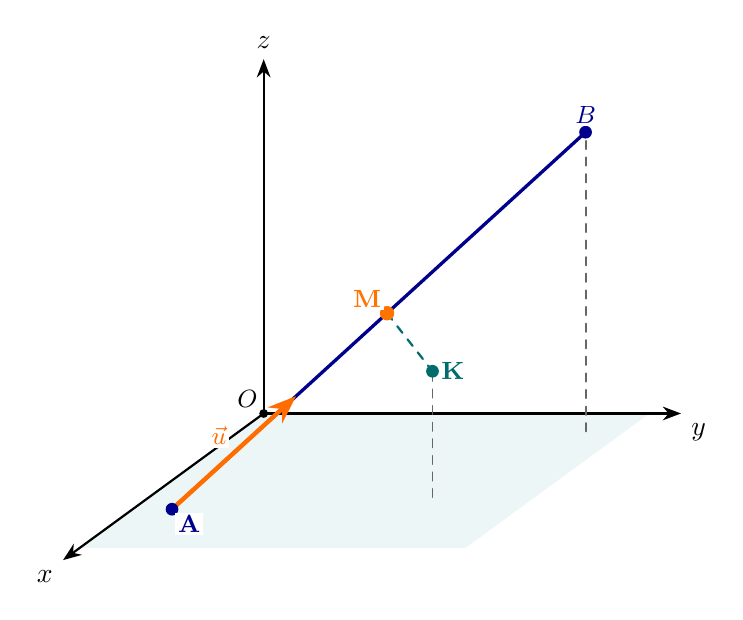
\begin{tikzpicture}[>=Stealth, line join=round, line cap=round,
    x={(-0.52cm,-0.38cm)}, y={(1cm,0cm)}, z={(0cm,1cm)}]
    \coordinate (O) at (0,0,0);
    \coordinate (A) at (3.2,0.5,0);
    \coordinate (B) at (0.6,4.4,3.8);
    \coordinate (Bxy) at (0.6,4.4,0);
    \coordinate (M) at ($(A)!0.52!(B)$);
    \coordinate (K) at (2.8,3.6,1.6);
    \coordinate (Kxy) at (2.8,3.6,0);

    % Mat dat Oxy
    \fill[teal!10, opacity=0.7] (0,0,0) -- (4.5,0,0) -- (4.5,4.9,0) -- (0,4.9,0) -- cycle;

    % 3 truc toa do Oxyz chuan SGK
    \draw[->, thick, black] (O) -- (4.9,0,0) node[below left] {$x$};
    \draw[->, thick, black] (O) -- (0,5.3,0) node[below right] {$y$};
    \draw[->, thick, black] (O) -- (0,0,4.5) node[above] {$z$};

    % Duong giong do cao cua ga B va tram K
    \draw[dashed, black!60, line width=0.7pt] (Bxy) -- (B);
    \draw[dashed, black!60, line width=0.7pt] (Kxy) -- (K);

    % Duong cap treo AB va vecto chi phuong
    \draw[very thick, blue!55!black] (A) -- (B);
    \draw[->, ultra thick, orange!85!red] (A) -- ($(A)!0.30!(B)$) node[midway, above left=1pt, fill=white, inner sep=1pt] {\small $\vec{u}$};
    \draw[dashed, thick, teal!85!black] (M) -- (K);

    % Chi ghi ten diem ngan gon (khong ghi toa do de tranh de chu)
    \fill[black] (O) circle (1.6pt) node[above left=1pt, fill=white, inner sep=1pt] {\small $O$};
    \fill[blue!55!black] (A) circle (2.3pt) node[below right=1pt, fill=white, inner sep=1pt] {\small $\mathbf{A}$};
    \fill[blue!55!black] (B) circle (2.3pt) node[above=2pt, fill=white, inner sep=1pt] {\small $B$};
    \fill[orange!90!red] (M) circle (2.6pt) node[above left=1pt, fill=white, inner sep=1pt] {\small $\mathbf{M}$};
    \fill[teal!85!black] (K) circle (2.3pt) node[right=2pt, fill=white, inner sep=1pt] {\small $\mathbf{K}$};
\end{tikzpicture}%
}
\end{minipage}

\end{enumerate}

% ==========================================
% PHẦN III
% ==========================================
\section*{\large PHẦN III. CÂU TRẮC NGHIỆM TRẢ LỜI NGẮN}
\textit{Thí sinh trả lời từ câu 1 đến câu 6. Điền đáp số theo quy chuẩn làm tròn được nêu trong từng câu.}

\begin{enumerate}[label=\textbf{Câu \arabic*:}, leftmargin=*]

\item \begin{minipage}[t]{0.55\linewidth}
Một cột đèn trang trí công viên có dạng hình lăng trụ tam giác đều $ABC.A'B'C'$ với độ dài cạnh đáy bằng $4\text{ dm}$ và độ dài cạnh bên bằng $9\text{ dm}$ (như hình vẽ). Người ta muốn căng một dải đèn LED bắt đầu từ đỉnh $A$ ở mặt đáy dưới, quấn một vòng áp sát quanh ba mặt bên của cột (lần lượt đi qua điểm $M$ trên cạnh bên $BB'$ và điểm $N$ trên cạnh bên $CC'$) rồi kết thúc tại đúng đỉnh $A'$ ở mặt đáy trên. Chiều dài ngắn nhất của dải đèn LED cần dùng bằng bao nhiêu đềximét ($\text{dm}$)?
\end{minipage}\hfill
\begin{minipage}[t]{0.42\linewidth}
\vspace{-0.4\baselineskip}
\centering
\resizebox{0.78\linewidth}{!}{%
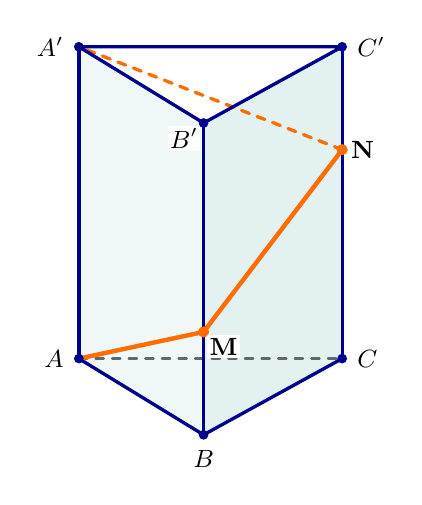
\begin{tikzpicture}[>=Stealth, line join=round, line cap=round, scale=0.88]
    \coordinate (A) at (0,0);
    \coordinate (B) at (1.8,-1.1);
    \coordinate (C) at (3.8,0);
    \coordinate (Ap) at (0,4.5);
    \coordinate (Bp) at (1.8,3.4);
    \coordinate (Cp) at (3.8,4.5);
    \coordinate (M) at ($(B)!0.33!(Bp)$);
    \coordinate (N) at ($(C)!0.67!(Cp)$);

    \fill[teal!10, opacity=0.6] (A) -- (B) -- (Bp) -- (Ap) -- cycle;
    \fill[teal!18, opacity=0.6] (B) -- (C) -- (Cp) -- (Bp) -- cycle;

    % Canh khuat AC va day M -> N -> A'
    \draw[dashed, thick, black!60] (A) -- (C);
    \draw[dashed, very thick, orange!85!red] (N) -- (Ap);

    % Cac canh thay cua lang tru
    \draw[very thick, blue!55!black] (A) -- (B) -- (C);
    \draw[very thick, blue!55!black] (Ap) -- (Bp) -- (Cp) -- cycle;
    \draw[very thick, blue!55!black] (A) -- (Ap);
    \draw[very thick, blue!55!black] (B) -- (Bp);
    \draw[very thick, blue!55!black] (C) -- (Cp);

    % Dai den LED A -> M -> N (net lien)
    \draw[ultra thick, orange!85!red] (A) -- (M) -- (N);

    \foreach \pt in {A,B,C,Ap,Bp,Cp} \fill[blue!55!black] (\pt) circle (2.0pt);
    \foreach \pt in {M,N} \fill[orange!85!red] (\pt) circle (2.3pt);

    \node[left=2pt] at (A) {\small $A$};
    \node[below=2pt] at (B) {\small $B$};
    \node[right=2pt] at (C) {\small $C$};
    \node[left=2pt] at (Ap) {\small $A'$};
    \node[below left=1pt, fill=white, inner sep=0.8pt] at (Bp) {\small $B'$};
    \node[right=2pt] at (Cp) {\small $C'$};
    \node[below right=1pt, fill=white, inner sep=1pt] at (M) {\small $\mathbf{M}$};
    \node[right=2pt, fill=white, inner sep=1pt] at (N) {\small $\mathbf{N}$};
\end{tikzpicture}%
}
\end{minipage}
\vspace{0.2cm}

\item \begin{minipage}[t]{0.55\linewidth}
Một chân đế bê tông trang trí có chiều cao $3\text{ m}$ được đặt trên mặt đất phẳng (như hình vẽ). Nếu cắt khối bê tông này bởi một mặt phẳng nằm ngang cách mặt đất $x\text{ mét}$ ($0 \le x \le 3$) thì mặt cắt thu được luôn là một hình chữ nhật (phần gạch chéo trên hình) có chiều dài bằng $(6 - x)\text{ mét}$ và chiều rộng bằng $(4 - x)\text{ mét}$. Thể tích của khối bê tông đó bằng bao nhiêu mét khối ($\text{m}^3$)?
\end{minipage}\hfill
\begin{minipage}[t]{0.42\linewidth}
\vspace{-0.4\baselineskip}
\centering
\resizebox{0.92\linewidth}{!}{%
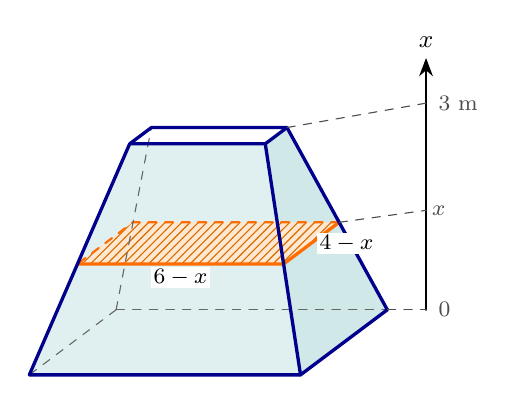
\begin{tikzpicture}[>=Stealth, line join=round, line cap=round,
    x={(-0.48cm,-0.36cm)}, y={(1cm,0cm)}, z={(0cm,1cm)}, scale=0.82]
    % Day duoi x=0: dai 6, rong 4 (scale 0.7 -> 4.2 x 2.8)
    \coordinate (A1) at (2.8,0,0);
    \coordinate (B1) at (2.8,4.2,0);
    \coordinate (C1) at (0,4.2,0);
    \coordinate (D1) at (0,0,0);

    % Day tren x=3: dai 3, rong 1 (scale 0.7 -> 2.1 x 0.7)
    \coordinate (A2) at (1.75,1.05,3.2);
    \coordinate (B2) at (1.75,3.15,3.2);
    \coordinate (C2) at (1.05,3.15,3.2);
    \coordinate (D2) at (1.05,1.05,3.2);

    % Thiet dien tai do cao x (trung gian t = 0.48)
    \coordinate (Am) at ($(A1)!0.48!(A2)$);
    \coordinate (Bm) at ($(B1)!0.48!(B2)$);
    \coordinate (Cm) at ($(C1)!0.48!(C2)$);
    \coordinate (Dm) at ($(D1)!0.48!(D2)$);

    % To mau nhe + gach cheo thiet dien
    \fill[teal!12] (A1) -- (B1) -- (B2) -- (A2) -- cycle;
    \fill[teal!18] (B1) -- (C1) -- (C2) -- (B2) -- cycle;
    \fill[orange!18] (Am) -- (Bm) -- (Cm) -- (Dm) -- cycle;
    \fill[pattern=north east lines, pattern color=orange!85!black] (Am) -- (Bm) -- (Cm) -- (Dm) -- cycle;
    \draw[very thick, orange!85!red] (Am) -- (Bm) -- (Cm);
    \draw[dashed, thick, orange!85!red] (Cm) -- (Dm) -- (Am);

    % Canh khuat va canh thay
    \draw[dashed, black!60] (D1) -- (A1);
    \draw[dashed, black!60] (D1) -- (C1);
    \draw[dashed, black!60] (D1) -- (D2);
    \draw[very thick, blue!55!black] (A1) -- (B1) -- (C1);
    \draw[very thick, blue!55!black] (A2) -- (B2) -- (C2) -- (D2) -- cycle;
    \draw[very thick, blue!55!black] (A1) -- (A2);
    \draw[very thick, blue!55!black] (B1) -- (B2);
    \draw[very thick, blue!55!black] (C1) -- (C2);

    % Truc do cao x
    \draw[->, thick, black] (0,4.8,0) -- (0,4.8,3.9) node[above] {\small $x$};
    \draw[dashed, black!70] (C1) -- (0,4.8,0) node[right=1pt] {\footnotesize $0$};
    \draw[dashed, black!70] (Cm) -- (0,4.8,1.54) node[right=1pt, fill=white, inner sep=1pt] {\footnotesize $x$};
    \draw[dashed, black!70] (C2) -- (0,4.8,3.2) node[right=1pt] {\footnotesize $3\text{ m}$};

    \node[below=1pt, fill=white, inner sep=0.8pt] at ($(Am)!0.5!(Bm)$) {\footnotesize $6 - x$};
    \node[right=2pt, fill=white, inner sep=0.8pt] at ($(Bm)!0.5!(Cm)$) {\footnotesize $4 - x$};
\end{tikzpicture}%
}
\end{minipage}
\vspace{0.2cm}

\item Nhà máy $A$ chuyên sản xuất một loại linh kiện bán dẫn cung cấp theo đơn đặt hàng hàng tháng cho đối tác. Nếu số lượng đặt hàng trong tháng là $x$ lô linh kiện ($1 \le x \le 150$) thì giá bán mỗi lô linh kiện là $p(x) = 200 - 0{,}5x$ (triệu đồng). Tổng chi phí để nhà máy sản xuất $x$ lô linh kiện trong tháng là $C(x) = 150 + 72x$ (triệu đồng). Ngoài ra, nhà máy phải nộp khoản thuế môi trường và phí quản lý bằng $10\%$ tổng doanh thu của tháng đó. Hỏi mỗi tháng nhà máy $A$ nên sản xuất và cung ứng bao nhiêu lô linh kiện để lợi nhuận ròng sau thuế thu được là lớn nhất?
\vspace{0.15cm}

\item \begin{minipage}[t]{0.55\linewidth}
Trong không gian $Oxyz$ (đơn vị trên mỗi trục tọa độ là mét), mặt phẳng $(Oxy)$ trùng với mặt đất. Một hệ thống ròng rọc vận chuyển vật liệu xây dựng gồm một dây cáp căng thẳng nối từ điểm neo $A(1; 2; 3)$ đến điểm neo $B(9; 10; 7)$ (như hình vẽ). Trên mặt đất $(Oxy)$, người ta cần đặt một trạm điều khiển tại điểm $M(a; b; 0)$ sao cho biểu thức $T = MA^2 + 3MB^2$ đạt giá trị nhỏ nhất. Tính giá trị của biểu thức $P = a + 2b$.
\end{minipage}\hfill
\begin{minipage}[t]{0.42\linewidth}
\vspace{-0.4\baselineskip}
\centering
\resizebox{0.92\linewidth}{!}{%
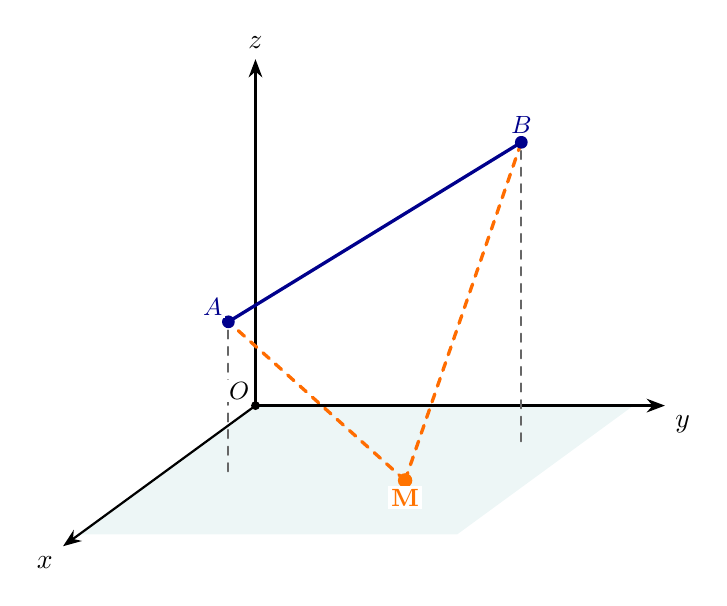
\begin{tikzpicture}[>=Stealth, line join=round, line cap=round,
    x={(-0.52cm,-0.38cm)}, y={(1cm,0cm)}, z={(0cm,1cm)}]
    \coordinate (O) at (0,0,0);
    \coordinate (A) at (2.2,0.8,1.9);
    \coordinate (Axy) at (2.2,0.8,0);
    \coordinate (B) at (1.2,4.0,3.8);
    \coordinate (Bxy) at (1.2,4.0,0);
    \coordinate (M) at (2.5,3.2,0);

    % Mat dat Oxy
    \fill[teal!10, opacity=0.7] (0,0,0) -- (4.3,0,0) -- (4.3,4.8,0) -- (0,4.8,0) -- cycle;

    % Truc Oxyz chuan SGK
    \draw[->, thick, black] (O) -- (4.7,0,0) node[below left] {$x$};
    \draw[->, thick, black] (O) -- (0,5.2,0) node[below right] {$y$};
    \draw[->, thick, black] (O) -- (0,0,4.4) node[above] {$z$};

    % Duong giong tu A, B xuong mat dat Oxy
    \draw[dashed, black!60, line width=0.7pt] (Axy) -- (A);
    \draw[dashed, black!60, line width=0.7pt] (Bxy) -- (B);

    % Day cap AB va khoang cach MA, MB
    \draw[very thick, blue!55!black] (A) -- (B);
    \draw[dashed, very thick, orange!85!red] (M) -- (A);
    \draw[dashed, very thick, orange!85!red] (M) -- (B);

    % Chi ghi ten diem O, A, B, M ngan gon (khong ghi toa do)
    \fill[black] (O) circle (1.6pt) node[above left=1pt, fill=white, inner sep=1pt] {\small $O$};
    \fill[blue!55!black] (A) circle (2.3pt) node[above left=1pt, fill=white, inner sep=1pt] {\small $A$};
    \fill[blue!55!black] (B) circle (2.3pt) node[above=2pt, fill=white, inner sep=1pt] {\small $B$};
    \fill[orange!90!red] (M) circle (2.6pt) node[below=2pt, fill=white, inner sep=1pt] {\small $\mathbf{M}$};
\end{tikzpicture}%
}
\end{minipage}
\vspace{0.2cm}

\item Để truyền một tín hiệu điều khiển (bit $0$ hoặc bit $1$) qua một kênh viễn thông có nhiễu, bộ phát chọn ngẫu nhiên bit $0$ hoặc bit $1$ với xác suất bằng nhau là $0{,}5$. Để chống nhiễu, bộ phát sử dụng mã lặp bộ ba: nếu muốn truyền bit $0$ thì gửi đi chuỗi $000$, nếu muốn truyền bit $1$ thì gửi đi chuỗi $111$. Khi đi qua kênh truyền, mỗi bit trong chuỗi có xác suất bị đảo ngược (từ $0$ thành $1$ hoặc từ $1$ thành $0$) độc lập với nhau và đều bằng $0{,}2$ (xác suất truyền đúng mỗi bit là $0{,}8$). Biết rằng đầu thu nhận được chuỗi ba bit là $110$, xác suất để tín hiệu gốc mà bộ phát muốn truyền đi là bit $1$ bằng bao nhiêu (viết kết quả dưới dạng số thập phân)?
\vspace{0.15cm}

\item \begin{minipage}[t]{0.55\linewidth}
Một cổng chào trang trí được thiết kế trên hệ trục tọa độ $Oxy$ (đơn vị trên mỗi trục là mét) có hình dạng giới hạn bởi hai đường parabol có phương trình $y = 9 - x^2$ và $y = 6 - \dfrac{2}{3}x^2$ cùng với trục hoành $Ox$ (với $y \ge 0$, như hình vẽ). Phần vòm phía trên (phần gạch chéo nằm giữa hai parabol) được ốp đá hoa cương với chi phí $2\text{ triệu đồng/m}^2$, còn phần khung lối đi phía dưới (phần tô đậm giới hạn bởi parabol thấp hơn và trục hoành) được lắp kính cường lực chống nắng với chi phí $1\text{ triệu đồng/m}^2$. Tổng chi phí để ốp đá hoa cương và lắp kính cường lực cho toàn bộ mặt cổng chào bằng bao nhiêu triệu đồng?
\end{minipage}\hfill
\begin{minipage}[t]{0.42\linewidth}
\vspace{-0.4\baselineskip}
\centering
\resizebox{0.92\linewidth}{!}{%
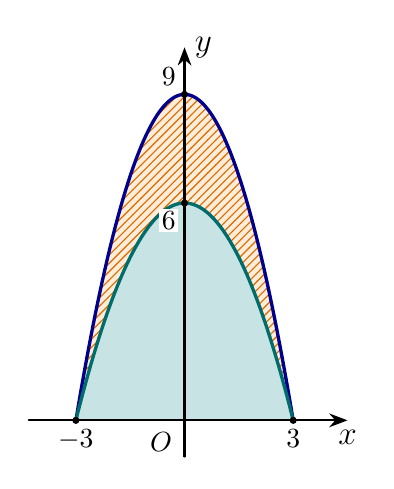
\begin{tikzpicture}[>=Stealth, line join=round, line cap=round, scale=0.46]
    % Phan vom gach cheo giua 2 parabol [-3, 3]
    \fill[orange!15]
        plot[domain=-3:3, samples=80] (\x, {9 - \x*\x})
        -- plot[domain=3:-3, samples=80] (\x, {6 - (2/3)*\x*\x}) -- cycle;
    \fill[pattern=north east lines, pattern color=orange!85!black]
        plot[domain=-3:3, samples=80] (\x, {9 - \x*\x})
        -- plot[domain=3:-3, samples=80] (\x, {6 - (2/3)*\x*\x}) -- cycle;

    % Phan khung loi di to dam duoi parabol thap hon [-3, 3]
    \fill[teal!22]
        plot[domain=-3:3, samples=80] (\x, {6 - (2/3)*\x*\x})
        -- (3,0) -- (-3,0) -- cycle;

    % Hai duong parabol (khong chu thich phuong trinh len duong cong de hoc sinh tu nhan biet)
    \draw[very thick, blue!55!black, domain=-3:3, samples=100] plot (\x, {9 - \x*\x});
    \draw[very thick, teal!85!black, domain=-3:3, samples=100] plot (\x, {6 - (2/3)*\x*\x});

    % Truc toa do Oxy chuan SGK
    \draw[->, thick, black] (-4.3,0) -- (4.5,0) node[below] {\large $x$};
    \draw[->, thick, black] (0,-1.0) -- (0,10.3) node[right] {\large $y$};
    \node[below left=1pt] at (0,0) {$O$};

    % Cac moc toa do tren truc
    \fill[black] (-3,0) circle (2.8pt) node[below=2pt, fill=white, inner sep=1pt] {$-3$};
    \fill[black] (3,0) circle (2.8pt) node[below=2pt, fill=white, inner sep=1pt] {$3$};
    \fill[black] (0,6) circle (2.8pt) node[below left=2pt, fill=white, inner sep=1pt] {$6$};
    \fill[black] (0,9) circle (2.8pt) node[above left=2pt, fill=white, inner sep=1pt] {$9$};
\end{tikzpicture}%
}
\end{minipage}

\end{enumerate}

\vspace{0.4cm}
\centerline{\textbf{--- HẾT ---}}

% ==========================================
% BẢNG ĐÁP ÁN TỔNG HỢP & LỜI GIẢI CHI TIẾT
% ==========================================
\newpage
\section*{\centering BẢNG ĐÁP ÁN TỔNG HỢP — ĐỀ SỐ 8}

\subsection*{Phần I. Trắc nghiệm nhiều phương án lựa chọn}
\begin{center}
\renewcommand{\arraystretch}{1.4}
\begin{tabular}{|*{6}{>{\centering\arraybackslash}p{2.1cm}|}}
\hline
\textbf{Câu 1} & \textbf{Câu 2} & \textbf{Câu 3} & \textbf{Câu 4} & \textbf{Câu 5} & \textbf{Câu 6} \\
\hline
B & D & A & C & B & A \\
\hline
\textbf{Câu 7} & \textbf{Câu 8} & \textbf{Câu 9} & \textbf{Câu 10} & \textbf{Câu 11} & \textbf{Câu 12} \\
\hline
D & C & A & D & C & B \\
\hline
\end{tabular}
\end{center}

\subsection*{Phần II. Trắc nghiệm Đúng/Sai}
\begin{center}
\renewcommand{\arraystretch}{1.4}
\begin{tabular}{|c|>{\centering\arraybackslash}p{3.0cm}|>{\centering\arraybackslash}p{3.0cm}|>{\centering\arraybackslash}p{3.0cm}|>{\centering\arraybackslash}p{3.0cm}|}
\hline
\textbf{Ý} & \textbf{Câu 1} & \textbf{Câu 2} & \textbf{Câu 3} & \textbf{Câu 4} \\
\hline
\textbf{a)} & Đúng & Đúng & Đúng & Đúng \\
\hline
\textbf{b)} & Đúng & Sai & Đúng & Đúng \\
\hline
\textbf{c)} & Sai & Đúng & Sai & Sai \\
\hline
\textbf{d)} & Đúng & Đúng & Đúng & Đúng \\
\hline
\end{tabular}
\end{center}

\subsection*{Phần III. Trắc nghiệm trả lời ngắn}
\begin{center}
\renewcommand{\arraystretch}{1.4}
\begin{tabular}{|*{6}{>{\centering\arraybackslash}p{2.1cm}|}}
\hline
\textbf{Câu 1} & \textbf{Câu 2} & \textbf{Câu 3} & \textbf{Câu 4} & \textbf{Câu 5} & \textbf{Câu 6} \\
\hline
15 & 36 & 120 & 23 & 0,8 & 48 \\
\hline
\end{tabular}
\end{center}

\vspace{0.4cm}
\section*{\centering HƯỚNG DẪN GIẢI CHI TIẾT}

\subsection*{PHẦN I. CÂU TRẮC NGHIỆM NHIỀU PHƯƠNG ÁN LỰA CHỌN}

\begin{enumerate}[label=\textbf{Câu \arabic*:}, leftmargin=*]

\item \textbf{Chọn B.}\\
Tập xác định: $D = \mathbb{R} \setminus \{1\}$. Ta viết lại hàm số dưới dạng:
$$y = \dfrac{x^2 - 3x + 5}{x - 1} = x - 2 + \dfrac{3}{x - 1}$$
Đồ thị $(C)$ có tiệm cận đứng là đường thẳng $x = 1$ và tiệm cận xiên là đường thẳng $y = x - 2$. Suy ra giao điểm của hai đường tiệm cận là $I(1; -1)$.\\
Ta có đạo hàm $y' = 1 - \dfrac{3}{(x - 1)^2}$. Tại $x_0 = 2$, ta có $y(2) = 3$ và $y'(2) = 1 - 3 = -2$.\\
Phương trình tiếp tuyến của $(C)$ tại điểm $M(2; 3)$ là:
$$y = -2(x - 2) + 3 \iff 2x + y - 7 = 0 \quad (\Delta)$$
Khoảng cách từ điểm $I(1; -1)$ đến tiếp tuyến $\Delta$ là:
$$d(I, \Delta) = \dfrac{|2\cdot 1 + (-1) - 7|}{\sqrt{2^2 + 1^2}} = \dfrac{6}{\sqrt{5}} = \dfrac{6\sqrt{5}}{5}.$$

\item \textbf{Chọn D.}\\
Phương trình đã cho tương đương với: $(3^x)^2 - 18\cdot 3^x + 27 = 0$.\\
Đặt $t = 3^x$ ($t > 0$), phương trình trở thành: $t^2 - 18t + 27 = 0$.\\
Vì $\Delta' = (-9)^2 - 27 = 54 > 0$, $S = t_1 + t_2 = 18 > 0$ và $P = t_1 t_2 = 27 > 0$ nên phương trình ẩn $t$ có hai nghiệm dương phân biệt $t_1, t_2$.\\
Theo định lí Vi-ét, ta có:
$$3^{x_1} \cdot 3^{x_2} = t_1 t_2 = 27 \iff 3^{x_1 + x_2} = 3^3 \iff x_1 + x_2 = 3.$$

\item \textbf{Chọn A.}\\
Đặt $A = \displaystyle\int_{1}^{3} f(x)\,\mathrm{d}x$ và $B = \displaystyle\int_{1}^{3} g(x)\,\mathrm{d}x$. Theo giả thiết ta có hệ phương trình:
$$\begin{cases} A + 3B = 10 \\ 2A - B = 6 \end{cases} \iff \begin{cases} A = 4 \\ B = 2 \end{cases}$$
Khi đó:
$$I = \int_{1}^{3} f(x)\,\mathrm{d}x + 2\int_{1}^{3} g(x)\,\mathrm{d}x + \int_{1}^{3} (-2x + 1)\,\mathrm{d}x = 4 + 2\cdot 2 + \left[-x^2 + x\right]_{1}^{3} = 8 + (-6 - 0) = 2.$$

\item \textbf{Chọn C.}\\
Mặt cầu $(S)$ tiếp xúc với mặt phẳng $(P): 2x - 2y + z + 3 = 0$ nên bán kính $R$ của mặt cầu bằng khoảng cách từ tâm $I(2; -1; 3)$ đến $(P)$:
$$R = d(I, (P)) = \dfrac{|2\cdot 2 - 2\cdot(-1) + 3 + 3|}{\sqrt{2^2 + (-2)^2 + 1^2}} = \dfrac{12}{3} = 4$$
Vậy phương trình mặt cầu $(S)$ là: $(x - 2)^2 + (y + 1)^2 + (z - 3)^2 = 16$.

\item \textbf{Chọn B.}\\
Gọi $A$ là biến cố ``Cuốn sách lấy ra do phân xưởng $A$ in'', suy ra $\overline{A} = B$ là biến cố ``Cuốn sách lấy ra do phân xưởng $B$ in''. Ta có $P(A) = 0{,}60$ và $P(B) = 0{,}40$.\\
Gọi $E$ là biến cố ``Cuốn sách lấy ra không đạt chuẩn chất lượng''. Ta có:
$$P(E \mid A) = 1 - 0{,}95 = 0{,}05; \quad P(E \mid B) = 1 - 0{,}90 = 0{,}10$$
Theo công thức xác suất toàn phần:
$$P(E) = P(A)\cdot P(E \mid A) + P(B)\cdot P(E \mid B) = 0{,}60\cdot 0{,}05 + 0{,}40\cdot 0{,}10 = 0{,}03 + 0{,}04 = 0{,}07$$
Theo công thức Bayes, xác suất cuốn sách không đạt chuẩn đó được in tại phân xưởng $A$ là:
$$P(A \mid E) = \dfrac{P(A)\cdot P(E \mid A)}{P(E)} = \dfrac{0{,}03}{0{,}07} = \dfrac{3}{7}.$$

\item \textbf{Chọn A.}\\
Cỡ mẫu $n = 6 + 10 + 12 + 10 + 2 = 40$.
\begin{itemize}
    \item Tứ phân vị thứ nhất $Q_1$: Ta có $\dfrac{n}{4} = 10$. Nhóm chứa $Q_1$ là nhóm $[15; 20)$ có $u_2 = 15$, $n_2 = 10$, $C_1 = 6$, độ dài nhóm $h = 5$:
    $$Q_1 = 15 + \dfrac{10 - 6}{10}\cdot 5 = 17.$$
    \item Tứ phân vị thứ ba $Q_3$: Ta có $\dfrac{3n}{4} = 30$. Tần số tích lũy của $3$ nhóm đầu là $6 + 10 + 12 = 28 < 30$, nên nhóm chứa $Q_3$ là nhóm $[25; 30)$ có $u_4 = 25$, $n_4 = 10$, $C_3 = 28$, $h = 5$:
    $$Q_3 = 25 + \dfrac{30 - 28}{10}\cdot 5 = 26.$$
\end{itemize}
Vậy khoảng tứ phân vị của mẫu số liệu ghép nhóm là $\Delta_Q = Q_3 - Q_1 = 26 - 17 = 9$.

\item \textbf{Chọn D.}\\
Trên đoạn $[1; e^2]$, hàm số $f(x) = x - 2\ln x$ liên tục và có đạo hàm:
$$f'(x) = 1 - \dfrac{2}{x} = 0 \iff x = 2 \in [1; e^2]$$
Tính giá trị của hàm số tại các điểm:
$$f(1) = 1; \quad f(2) = 2 - 2\ln 2 \approx 0{,}614; \quad f(e^2) = e^2 - 2\ln(e^2) = e^2 - 4 \approx 3{,}389$$
Vậy $\max\limits_{[1; e^2]} f(x) = f(e^2) = e^2 - 4$.

\item \textbf{Chọn C.}\\
Phương trình hoành độ giao điểm của đường cong và trục hoành:
$$\sqrt{4x - x^2} = 0 \iff 4x - x^2 = 0 \iff x = 0 \text{ hoặc } x = 4$$
Thể tích khối tròn xoay khi quay $(H)$ quanh trục $Ox$ là:
$$V = \pi \int_{0}^{4} (4x - x^2)\,\mathrm{d}x = \pi \left[2x^2 - \dfrac{x^3}{3}\right]_{0}^{4} = \pi \left(32 - \dfrac{64}{3}\right) = \dfrac{32\pi}{3}.$$

\item \textbf{Chọn A.}\\
Đường thẳng $d$ có vectơ chỉ phương $\vec{u}_d = (2; -1; 2)$ và mặt phẳng $(P)$ có vectơ pháp tuyến $\vec{n}_P = (2; -1; -2)$.\\
Ta có:
$$\sin(d, (P)) = \dfrac{|\vec{u}_d \cdot \vec{n}_P|}{|\vec{u}_d| \cdot |\vec{n}_P|} = \dfrac{|2\cdot 2 + (-1)\cdot(-1) + 2\cdot(-2)|}{\sqrt{2^2 + (-1)^2 + 2^2}\cdot\sqrt{2^2 + (-1)^2 + (-2)^2}} = \dfrac{|4 + 1 - 4|}{3 \cdot 3} = \dfrac{1}{9}.$$

\item \textbf{Chọn D.}\\
Gọi $q > 0$ là công bội của cấp số nhân $(u_n)$. Ta có:
$$u_3 + u_4 = q^2(u_1 + u_2) \implies 108 = 12q^2 \implies q^2 = 9 \implies q = 3 \text{ (do } q > 0\text{)}$$
Thay $q = 3$ vào $u_1(1 + q) = 12 \implies 4u_1 = 12 \implies u_1 = 3$.\\
Vậy số hạng thứ $5$ là $u_5 = u_1 \cdot q^4 = 3 \cdot 3^4 = 243$.

\item \textbf{Chọn C.}\\
Vì $SA, AB, AD$ đôi một vuông góc tại $A$ nên khoảng cách $d$ từ điểm $A$ đến mặt phẳng $(SBD)$ được tính bởi hệ thức trong tứ diện vuông $A.SBD$:
$$\dfrac{1}{d^2} = \dfrac{1}{SA^2} + \dfrac{1}{AB^2} + \dfrac{1}{AD^2} = \dfrac{25}{144} + \dfrac{1}{9} + \dfrac{1}{16} = \dfrac{25 + 16 + 9}{144} = \dfrac{50}{144}$$
Suy ra $d = \dfrac{12}{\sqrt{50}} = \dfrac{12}{5\sqrt{2}} = \dfrac{6\sqrt{2}}{5}$.

\item \textbf{Chọn B.}\\
Số phần tử của không gian mẫu là $n(\Omega) = C_{20}^{3} = 1140$.\\
Ba số nguyên dương phân biệt $a < b < c$ lập thành một cấp số cộng khi và chỉ khi $a + c = 2b$, tức là $a$ và $c$ có cùng tính chẵn lẻ (ứng với mỗi cặp $(a, c)$ cùng chẵn hoặc cùng lẻ sẽ xác định duy nhất số hạng ở giữa $b = \dfrac{a+c}{2}$).\\
Từ $1$ đến $20$ có $10$ số chẵn và $10$ số lẻ, do đó số bộ $3$ tấm thẻ lập thành cấp số cộng là:
$$n(A) = C_{10}^{2} + C_{10}^{2} = 45 + 45 = 90$$
Xác suất cần tìm là $P(A) = \dfrac{90}{1140} = \dfrac{3}{38}$.

\end{enumerate}

\subsection*{PHẦN II. CÂU TRẮC NGHIỆM ĐÚNG/SAI}

\begin{enumerate}[label=\textbf{Câu \arabic*:}, leftmargin=*]

\item \textbf{Đáp án: a) Đúng \quad b) Đúng \quad c) Sai \quad d) Đúng}
\begin{itemize}
    \item \textbf{Ý a) Đúng:} Thay $t = 0 \implies C(0) = 0\text{ mg/lít}$; thay $t = 2 \implies C(2) = \dfrac{12}{4 + 4} = 1{,}5\text{ mg/lít}$.
    \item \textbf{Ý b) Đúng:} Áp dụng quy tắc đạo hàm thương:
    $$C'(t) = \dfrac{6(t^2 + 4) - 6t(2t)}{(t^2 + 4)^2} = \dfrac{24 - 6t^2}{(t^2 + 4)^2}.$$
    \item \textbf{Ý c) Sai:} Cho $C'(t) = 0 \iff 24 - 6t^2 = 0 \iff t = 2$ (vì $t \ge 0$). Hàm số đồng biến trên $[0; 2]$ và nghịch biến trên $(2; +\infty)$. Do đó nồng độ thuốc chỉ tăng trong $2$ giờ đầu rồi giảm dần từ giờ thứ $2$ trở đi.
    \item \textbf{Ý d) Đúng:} Giải bất phương trình:
    $$C(t) \ge 1{,}2 \iff \dfrac{6t}{t^2 + 4} \ge \dfrac{6}{5} \iff t^2 - 5t + 4 \le 0 \iff 1 \le t \le 4$$
    Vậy tổng thời gian thuốc phát huy hiệu quả điều trị tốt nhất là $4 - 1 = 3$ giờ.
\end{itemize}

\item \textbf{Đáp án: a) Đúng \quad b) Sai \quad c) Đúng \quad d) Đúng}
\begin{itemize}
    \item \textbf{Ý a) Đúng:} Trong $0{,}5$ giây phản ứng, xe đi được quãng đường $s_1 = 24 \cdot 0{,}5 = 12\text{ m}$.
    \item \textbf{Ý b) Sai:} Khi xe dừng hẳn thì $v(t) = 0 \iff 24 - 6t^2 = 0 \iff t = 2$ giây (do $t \ge 0$).
    \item \textbf{Ý c) Đúng:} Quãng đường xe đi được từ lúc bắt đầu đạp phanh đến khi dừng hẳn là:
    $$s_2 = \int_{0}^{2} (24 - 6t^2)\,\mathrm{d}t = \left[24t - 2t^3\right]_{0}^{2} = 48 - 16 = 32\text{ m}.$$
    \item \textbf{Ý d) Đúng:} Tổng quãng đường xe đã di chuyển từ lúc phát hiện chướng ngại vật đến khi dừng hẳn là $s = s_1 + s_2 = 12 + 32 = 44\text{ m} < 65\text{ m}$. Khi dừng hẳn, đầu xe còn cách chướng ngại vật $65 - 44 = 21\text{ m}$.
\end{itemize}

\item \textbf{Đáp án: a) Đúng \quad b) Đúng \quad c) Sai \quad d) Đúng}
\begin{itemize}
    \item \textbf{Ý a) Đúng:} Vì gói tin thứ nhất truyền qua Kênh $A$ nên xác suất gói tin thứ hai chuyển sang Kênh $B$ là $P(B_2) = 0{,}30$ và giữ nguyên ở Kênh $A$ là $P(A_2) = 0{,}70$.
    \item \textbf{Ý b) Đúng:} Xác suất cả gói tin thứ hai và thứ ba đều truyền qua Kênh $A$ là:
    $$P(A_2 \cap A_3) = P(A_2)\cdot P(A_3 \mid A_2) = 0{,}70 \cdot 0{,}70 = 0{,}49.$$
    \item \textbf{Ý c) Sai:} Theo công thức xác suất toàn phần, xác suất gói tin thứ ba truyền qua Kênh $A$ là:
    $$P(A_3) = P(A_2)\cdot P(A_3 \mid A_2) + P(B_2)\cdot P(A_3 \mid B_2) = 0{,}70\cdot 0{,}70 + 0{,}30\cdot 0{,}60 = 0{,}49 + 0{,}18 = 0{,}67.$$
    \item \textbf{Ý d) Đúng:} Theo công thức Bayes:
    $$P(B_2 \mid A_3) = \dfrac{P(B_2)\cdot P(A_3 \mid B_2)}{P(A_3)} = \dfrac{0{,}18}{0{,}67} = \dfrac{18}{67}.$$
\end{itemize}

\item \textbf{Đáp án: a) Đúng \quad b) Đúng \quad c) Sai \quad d) Đúng}
\begin{itemize}
    \item \textbf{Ý a) Đúng:} Đường cáp đi qua $A(10; 3; 0)$ và có vectơ chỉ phương $\vec{u} = (2; -2; 1)$ nên có phương trình chính tắc là $\dfrac{x - 10}{2} = \dfrac{y - 3}{-2} = \dfrac{z}{1}$.
    \item \textbf{Ý b) Đúng:} Ta có $|\vec{u}| = \sqrt{2^2 + (-2)^2 + 1^2} = 3$. Vectơ vận tốc của cabin có độ lớn $v = 6\text{ m/s}$ và cùng hướng với $\vec{u}$ là:
    $$\vec{v} = \dfrac{v}{|\vec{u}|}\vec{u} = \dfrac{6}{3}(2; -2; 1) = (4; -4; 2)$$
    Do đó sau $t$ giây, tọa độ cabin là $M(10 + 4t;\ 3 - 4t;\ 2t)$.
    \item \textbf{Ý c) Sai:} Tại ga đích $B$ có $z_B = 120 \implies 2t = 120 \iff t = 60$ giây.
    \item \textbf{Ý d) Đúng:} Ta có $\overrightarrow{KM} = (4t - 45;\ -4t + 35;\ 2t - 20)$. Khi đó:
    $$KM^2 = (4t - 45)^2 + (-4t + 35)^2 + (2t - 20)^2 = 36t^2 - 720t + 3650 = 36(t - 10)^2 + 50 \ge 50$$
    Dấu ``$=$'' xảy ra khi $t = 10$ giây. Vậy khoảng cách ngắn nhất từ cabin $M$ đến trạm phát sóng $K$ là $KM_{\min} = \sqrt{50} = 5\sqrt{2}\text{ m}$.
\end{itemize}

\end{enumerate}

\subsection*{PHẦN III. CÂU TRẮC NGHIỆM TRẢ LỜI NGẮN}

\begin{enumerate}[label=\textbf{Câu \arabic*:}, leftmargin=*]

\item \textbf{Đáp số: 15}\\
Trải phẳng ba mặt bên $(ABB'A')$, $(BCC'B')$ và $(CAA'C')$ của hình lăng trụ tam giác đều cùng nằm trên một mặt phẳng, ta thu được một hình chữ nhật có chiều rộng bằng chu vi đáy $3 \times 4 = 12\text{ dm}$ và chiều cao bằng độ dài cạnh bên $9\text{ dm}$.\\
Quãng đường của dải đèn LED từ $A$ qua $M, N$ đến $A'$ có độ dài ngắn nhất khi các điểm $A, M, N, A'$ trên hình trải phẳng thẳng hàng, tức là bằng độ dài đường chéo của hình chữ nhật:
$$L_{\min} = \sqrt{12^2 + 9^2} = \sqrt{144 + 81} = \sqrt{225} = 15\text{ (dm)}.$$

\item \textbf{Đáp số: 36}\\
Diện tích của thiết diện mặt cắt hình chữ nhật tại vị trí cách mặt đất $x\text{ mét}$ ($0 \le x \le 3$) là:
$$S(x) = (6 - x)(4 - x) = x^2 - 10x + 24\text{ (m}^2\text{)}$$
Thể tích của khối bê tông là:
$$V = \int_{0}^{3} S(x)\,\mathrm{d}x = \int_{0}^{3} (x^2 - 10x + 24)\,\mathrm{d}x = \left[\dfrac{x^3}{3} - 5x^2 + 24x\right]_{0}^{3} = 9 - 45 + 72 = 36\text{ (m}^3\text{)}.$$

\item \textbf{Đáp số: 120}\\
Tổng doanh thu khi bán $x$ lô linh kiện là: $R(x) = x\cdot p(x) = 200x - 0{,}5x^2$ (triệu đồng).\\
Sau khi nộp $10\%$ thuế trên tổng doanh thu, phần doanh thu còn lại là $0{,}9R(x) = 180x - 0{,}45x^2$.\\
Hàm lợi nhuận ròng sau thuế là:
$$L(x) = 0{,}9R(x) - C(x) = (180x - 0{,}45x^2) - (150 + 72x) = -0{,}45x^2 + 108x - 150$$
Ta có $L'(x) = -0{,}9x + 108 = 0 \iff x = 120 \in [1; 150]$.\\
Vì $L''(x) = -0{,}9 < 0$ nên lợi nhuận ròng đạt giá trị lớn nhất khi nhà máy sản xuất $x = 120$ lô linh kiện mỗi tháng.

\item \textbf{Đáp số: 23}\\
Với $M(a; b; 0) \in (Oxy)$, ta có:
$$T = MA^2 + 3MB^2 = \left[(a - 1)^2 + (b - 2)^2 + 3^2\right] + 3\left[(a - 9)^2 + (b - 10)^2 + 7^2\right]$$
$$= 4(a^2 - 14a) + 4(b^2 - 16b) + 560 = 4(a - 7)^2 + 4(b - 8)^2 + 108 \ge 108$$
Biểu thức $T$ đạt giá trị nhỏ nhất khi và chỉ khi $a = 7$ và $b = 8$.\\
Khi đó giá trị của biểu thức $P = a + 2b = 7 + 2\cdot 8 = 23$.

\item \textbf{Đáp số: 0,8}\\
Gọi $B_1$ là biến cố ``Bộ phát muốn truyền bit $1$ (gửi chuỗi $111$)'' và $B_0$ là biến cố ``Bộ phát muốn truyền bit $0$ (gửi chuỗi $000$)''. Ta có $P(B_1) = P(B_0) = 0{,}5$.\\
Gọi $E$ là biến cố ``Đầu thu nhận được chuỗi $110$''.
\begin{itemize}
    \item Nếu bộ phát gửi $111$, để nhận được $110$ thì hai bit đầu phải truyền đúng và bit thứ ba bị lỗi:
    $$P(E \mid B_1) = 0{,}8 \times 0{,}8 \times 0{,}2 = 0{,}128.$$
    \item Nếu bộ phát gửi $000$, để nhận được $110$ thì hai bit đầu bị lỗi và bit thứ ba truyền đúng:
    $$P(E \mid B_0) = 0{,}2 \times 0{,}2 \times 0{,}8 = 0{,}032.$$
\end{itemize}
Theo công thức Bayes, xác suất tín hiệu gốc muốn truyền đi là bit $1$ bằng:
$$P(B_1 \mid E) = \dfrac{0{,}5 \times 0{,}128}{0{,}5 \times 0{,}128 + 0{,}5 \times 0{,}032} = \dfrac{0{,}128}{0{,}160} = \dfrac{4}{5} = 0{,}8.$$

\item \textbf{Đáp số: 48}\\
Quan sát đồ thị và phương trình hai parabol, cả hai parabol đều cắt trục hoành tại hai điểm có hoành độ $x = -3$ và $x = 3$:
\begin{itemize}
    \item Parabol đi qua đỉnh $(0; 9)$ là đường cong phía trên: $y = 9 - x^2$.
    \item Parabol đi qua đỉnh $(0; 6)$ là đường cong phía dưới: $y = 6 - \dfrac{2}{3}x^2$.
\end{itemize}
Diện tích phần vòm gạch chéo (ốp đá hoa cương) là:
$$S_1 = \int_{-3}^{3} \left[(9 - x^2) - \left(6 - \dfrac{2}{3}x^2\right)\right]\mathrm{d}x = \int_{-3}^{3} \left(3 - \dfrac{1}{3}x^2\right)\mathrm{d}x = \left[3x - \dfrac{x^3}{9}\right]_{-3}^{3} = 12\text{ (m}^2\text{)}$$
Diện tích phần khung lối đi tô đậm (lắp kính cường lực) là:
$$S_2 = \int_{-3}^{3} \left(6 - \dfrac{2}{3}x^2\right)\mathrm{d}x = \left[6x - \dfrac{2x^3}{9}\right]_{-3}^{3} = 24\text{ (m}^2\text{)}$$
Tổng chi phí thi công là: $12 \times 2 + 24 \times 1 = 48$ (triệu đồng).

\end{enumerate}

\end{document}
